\documentclass[1p]{elsarticle_modified}
%\bibliographystyle{elsarticle-num}

%\usepackage[colorlinks]{hyperref}
%\usepackage{abbrmath_seonhwa} %\Abb, \Ascr, \Acal ,\Abf, \Afrak
\usepackage{amsfonts}
\usepackage{amssymb}
\usepackage{amsmath}
\usepackage{amsthm}
\usepackage{scalefnt}
\usepackage{amsbsy}
\usepackage{kotex}
\usepackage{caption}
\usepackage{subfig}
\usepackage{color}
\usepackage{graphicx}
\usepackage{xcolor} %% white, black, red, green, blue, cyan, magenta, yellow
\usepackage{float}
\usepackage{setspace}
\usepackage{hyperref}

\usepackage{tikz}
\usetikzlibrary{arrows}

\usepackage{multirow}
\usepackage{array} % fixed length table
\usepackage{hhline}

%%%%%%%%%%%%%%%%%%%%%
\makeatletter
\renewcommand*\env@matrix[1][\arraystretch]{%
	\edef\arraystretch{#1}%
	\hskip -\arraycolsep
	\let\@ifnextchar\new@ifnextchar
	\array{*\c@MaxMatrixCols c}}
\makeatother %https://tex.stackexchange.com/questions/14071/how-can-i-increase-the-line-spacing-in-a-matrix
%%%%%%%%%%%%%%%

\usepackage[normalem]{ulem}

\newcommand{\msout}[1]{\ifmmode\text{\sout{\ensuremath{#1}}}\else\sout{#1}\fi}
%SOURCE: \msout is \stkout macro in https://tex.stackexchange.com/questions/20609/strikeout-in-math-mode

\newcommand{\cancel}[1]{
	\ifmmode
	{\color{red}\msout{#1}}
	\else
	{\color{red}\sout{#1}}
	\fi
}

\newcommand{\add}[1]{
	{\color{blue}\uwave{#1}}
}

\newcommand{\replace}[2]{
	\ifmmode
	{\color{red}\msout{#1}}{\color{blue}\uwave{#2}}
	\else
	{\color{red}\sout{#1}}{\color{blue}\uwave{#2}}
	\fi
}

\newcommand{\Sol}{\mathcal{S}} %segment
\newcommand{\D}{D} %diagram
\newcommand{\A}{\mathcal{A}} %arc


%%%%%%%%%%%%%%%%%%%%%%%%%%%%%5 test

\def\sl{\operatorname{\textup{SL}}(2,\Cbb)}
\def\psl{\operatorname{\textup{PSL}}(2,\Cbb)}
\def\quan{\mkern 1mu \triangleright \mkern 1mu}

\theoremstyle{definition}
\newtheorem{thm}{Theorem}[section]
\newtheorem{prop}[thm]{Proposition}
\newtheorem{lem}[thm]{Lemma}
\newtheorem{ques}[thm]{Question}
\newtheorem{cor}[thm]{Corollary}
\newtheorem{defn}[thm]{Definition}
\newtheorem{exam}[thm]{Example}
\newtheorem{rmk}[thm]{Remark}
\newtheorem{alg}[thm]{Algorithm}

\newcommand{\I}{\sqrt{-1}}
\begin{document}

%\begin{frontmatter}
%
%\title{Boundary parabolic representations of knots up to 8 crossings}
%
%%% Group authors per affiliation:
%\author{Yunhi Cho} 
%\address{Department of Mathematics, University of Seoul, Seoul, Korea}
%\ead{yhcho@uos.ac.kr}
%
%
%\author{Seonhwa Kim} %\fnref{s_kim}}
%\address{Center for Geometry and Physics, Institute for Basic Science, Pohang, 37673, Korea}
%\ead{ryeona17@ibs.re.kr}
%
%\author{Hyuk Kim}
%\address{Department of Mathematical Sciences, Seoul National University, Seoul 08826, Korea}
%\ead{hyukkim@snu.ac.kr}
%
%\author{Seokbeom Yoon}
%\address{Department of Mathematical Sciences, Seoul National University, Seoul, 08826,  Korea}
%\ead{sbyoon15@snu.ac.kr}
%
%\begin{abstract}
%We find all boundary parabolic representation of knots up to 8 crossings.
%
%\end{abstract}
%\begin{keyword}
%    \MSC[2010] 57M25 
%\end{keyword}
%
%\end{frontmatter}

%\linenumbers
%\tableofcontents
%
\newcommand\colored[1]{\textcolor{white}{\rule[-0.35ex]{0.8em}{1.4ex}}\kern-0.8em\color{red} #1}%
%\newcommand\colored[1]{\textcolor{white}{ #1}\kern-2.17ex	\textcolor{white}{ #1}\kern-1.81ex	\textcolor{white}{ #1}\kern-2.15ex\color{red}#1	}

{\Large $\underline{12a_{0241}~(K12a_{0241})}$}

\setlength{\tabcolsep}{10pt}
\renewcommand{\arraystretch}{1.6}
\vspace{1cm}\begin{tabular}{m{100pt}>{\centering\arraybackslash}m{274pt}}
\multirow{5}{120pt}{
	\centering
	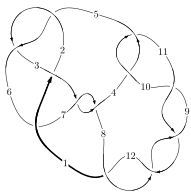
\includegraphics[width=112pt]{../../../GIT/diagram.site/Diagrams/png/1042_12a_0241.png}\\
\ \ \ A knot diagram\footnotemark}&
\allowdisplaybreaks
\textbf{Linearized knot diagam} \\
\cline{2-2}
 &
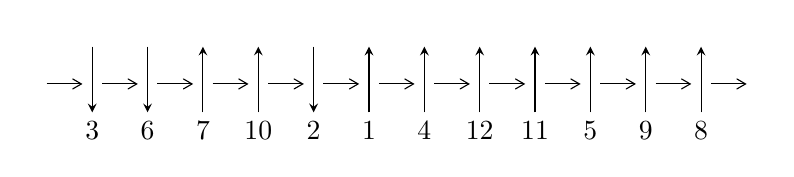
\begin{tikzpicture}[x=20pt, y=17pt]
	% nodes
	\node (C0) at (0, 0) {};
	\node (C1) at (1, 0) {};
	\node (C1U) at (1, +1) {};
	\node (C1D) at (1, -1) {3};

	\node (C2) at (2, 0) {};
	\node (C2U) at (2, +1) {};
	\node (C2D) at (2, -1) {6};

	\node (C3) at (3, 0) {};
	\node (C3U) at (3, +1) {};
	\node (C3D) at (3, -1) {7};

	\node (C4) at (4, 0) {};
	\node (C4U) at (4, +1) {};
	\node (C4D) at (4, -1) {10};

	\node (C5) at (5, 0) {};
	\node (C5U) at (5, +1) {};
	\node (C5D) at (5, -1) {2};

	\node (C6) at (6, 0) {};
	\node (C6U) at (6, +1) {};
	\node (C6D) at (6, -1) {1};

	\node (C7) at (7, 0) {};
	\node (C7U) at (7, +1) {};
	\node (C7D) at (7, -1) {4};

	\node (C8) at (8, 0) {};
	\node (C8U) at (8, +1) {};
	\node (C8D) at (8, -1) {12};

	\node (C9) at (9, 0) {};
	\node (C9U) at (9, +1) {};
	\node (C9D) at (9, -1) {11};

	\node (C10) at (10, 0) {};
	\node (C10U) at (10, +1) {};
	\node (C10D) at (10, -1) {5};

	\node (C11) at (11, 0) {};
	\node (C11U) at (11, +1) {};
	\node (C11D) at (11, -1) {9};

	\node (C12) at (12, 0) {};
	\node (C12U) at (12, +1) {};
	\node (C12D) at (12, -1) {8};
	\node (C13) at (13, 0) {};

	% arrows
	\draw[->,>={angle 60}]
	(C0) edge (C1) (C1) edge (C2) (C2) edge (C3) (C3) edge (C4) (C4) edge (C5) (C5) edge (C6) (C6) edge (C7) (C7) edge (C8) (C8) edge (C9) (C9) edge (C10) (C10) edge (C11) (C11) edge (C12) (C12) edge (C13) ;	\draw[->,>=stealth]
	(C1U) edge (C1D) (C2U) edge (C2D) (C3D) edge (C3U) (C4D) edge (C4U) (C5U) edge (C5D) (C6D) edge (C6U) (C7D) edge (C7U) (C8D) edge (C8U) (C9D) edge (C9U) (C10D) edge (C10U) (C11D) edge (C11U) (C12D) edge (C12U) ;
	\end{tikzpicture} \\
\hhline{~~} \\& 
\textbf{Solving Sequence} \\ \cline{2-2} 
 &
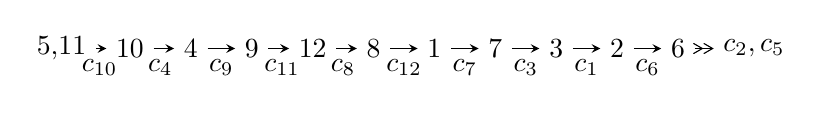
\begin{tikzpicture}[x=22pt, y=7pt]
	% node
	\node (A0) at (-1/8, 0) {5,11};
	\node (A1) at (1, 0) {10};
	\node (A2) at (2, 0) {4};
	\node (A3) at (3, 0) {9};
	\node (A4) at (4, 0) {12};
	\node (A5) at (5, 0) {8};
	\node (A6) at (6, 0) {1};
	\node (A7) at (7, 0) {7};
	\node (A8) at (8, 0) {3};
	\node (A9) at (9, 0) {2};
	\node (A10) at (10, 0) {6};
	\node (C1) at (1/2, -1) {$c_{10}$};
	\node (C2) at (3/2, -1) {$c_{4}$};
	\node (C3) at (5/2, -1) {$c_{9}$};
	\node (C4) at (7/2, -1) {$c_{11}$};
	\node (C5) at (9/2, -1) {$c_{8}$};
	\node (C6) at (11/2, -1) {$c_{12}$};
	\node (C7) at (13/2, -1) {$c_{7}$};
	\node (C8) at (15/2, -1) {$c_{3}$};
	\node (C9) at (17/2, -1) {$c_{1}$};
	\node (C10) at (19/2, -1) {$c_{6}$};
	\node (A11) at (45/4, 0) {$c_{2},c_{5}$};

	% edge
	\draw[->,>=stealth]	
	(A0) edge (A1) (A1) edge (A2) (A2) edge (A3) (A3) edge (A4) (A4) edge (A5) (A5) edge (A6) (A6) edge (A7) (A7) edge (A8) (A8) edge (A9) (A9) edge (A10) ;
	\draw[->>,>={angle 60}]	
	(A10) edge (A11);
\end{tikzpicture} \\ 

\end{tabular} \\

\footnotetext{
The image of knot diagram is generated by the software ``\textbf{Draw programme}" developed by Andrew Bartholomew(\url{http://www.layer8.co.uk/maths/draw/index.htm\#Running-draw}), where we modified some parts for our purpose(\url{https://github.com/CATsTAILs/LinksPainter}).
}\phantom \\ \newline 
\centering \textbf{Ideals for irreducible components\footnotemark of $X_{\text{par}}$} 
 
\begin{align*}
I^u_{1}&=\langle 
u^{63}- u^{62}+\cdots+2 u^2-1\rangle \\
\\
\end{align*}
\raggedright * 1 irreducible components of $\dim_{\mathbb{C}}=0$, with total 63 representations.\\
\footnotetext{All coefficients of polynomials are rational numbers. But the coefficients are sometimes approximated in decimal forms when there is not enough margin.}
\newpage
\renewcommand{\arraystretch}{1}
\centering \section*{I. $I^u_{1}= \langle u^{63}- u^{62}+\cdots+2 u^2-1 \rangle$}
\flushleft \textbf{(i) Arc colorings}\\
\begin{tabular}{m{7pt} m{180pt} m{7pt} m{180pt} }
\flushright $a_{5}=$&$\begin{pmatrix}0\\u\end{pmatrix}$ \\
\flushright $a_{11}=$&$\begin{pmatrix}1\\0\end{pmatrix}$ \\
\flushright $a_{10}=$&$\begin{pmatrix}1\\u^2\end{pmatrix}$ \\
\flushright $a_{4}=$&$\begin{pmatrix}- u\\- u^3+u\end{pmatrix}$ \\
\flushright $a_{9}=$&$\begin{pmatrix}- u^2+1\\u^2\end{pmatrix}$ \\
\flushright $a_{12}=$&$\begin{pmatrix}u^4- u^2+1\\- u^4\end{pmatrix}$ \\
\flushright $a_{8}=$&$\begin{pmatrix}- u^6+u^4-2 u^2+1\\u^6+u^2\end{pmatrix}$ \\
\flushright $a_{1}=$&$\begin{pmatrix}u^8- u^6+3 u^4-2 u^2+1\\- u^8-2 u^4\end{pmatrix}$ \\
\flushright $a_{7}=$&$\begin{pmatrix}- u^{10}+u^8-4 u^6+3 u^4-3 u^2+1\\- u^{12}+2 u^{10}-4 u^8+6 u^6-3 u^4+2 u^2\end{pmatrix}$ \\
\flushright $a_{3}=$&$\begin{pmatrix}u^{19}-2 u^{17}+8 u^{15}-12 u^{13}+21 u^{11}-22 u^9+20 u^7-12 u^5+5 u^3-2 u\\u^{21}-3 u^{19}+\cdots-3 u^3+u\end{pmatrix}$ \\
\flushright $a_{2}=$&$\begin{pmatrix}u^{48}-5 u^{46}+\cdots-4 u^2+1\\u^{50}-6 u^{48}+\cdots-10 u^4+u^2\end{pmatrix}$ \\
\flushright $a_{6}=$&$\begin{pmatrix}u^{28}-3 u^{26}+\cdots-5 u^2+1\\- u^{28}+2 u^{26}+\cdots-3 u^4+2 u^2\end{pmatrix}$\\&\end{tabular}
\flushleft \textbf{(ii) Obstruction class $= -1$}\\~\\
\flushleft \textbf{(iii) Cusp Shapes $= 4 u^{62}-28 u^{60}+\cdots+16 u+6$}\\~\\
\newpage\renewcommand{\arraystretch}{1}
\flushleft \textbf{(iv) u-Polynomials at the component}\newline \\
\begin{tabular}{m{50pt}|m{274pt}}
Crossings & \hspace{64pt}u-Polynomials at each crossing \\
\hline $$\begin{aligned}c_{1}\end{aligned}$$&$\begin{aligned}
&u^{63}+29 u^{62}+\cdots+4 u+1
\end{aligned}$\\
\hline $$\begin{aligned}c_{2},c_{5}\end{aligned}$$&$\begin{aligned}
&u^{63}+u^{62}+\cdots+2 u-1
\end{aligned}$\\
\hline $$\begin{aligned}c_{3},c_{7}\end{aligned}$$&$\begin{aligned}
&u^{63}- u^{62}+\cdots+420 u-97
\end{aligned}$\\
\hline $$\begin{aligned}c_{4},c_{10}\end{aligned}$$&$\begin{aligned}
&u^{63}- u^{62}+\cdots+2 u^2-1
\end{aligned}$\\
\hline $$\begin{aligned}c_{6}\end{aligned}$$&$\begin{aligned}
&u^{63}+3 u^{62}+\cdots+34 u-5
\end{aligned}$\\
\hline $$\begin{aligned}c_{8},c_{9},c_{11}\\c_{12}\end{aligned}$$&$\begin{aligned}
&u^{63}-13 u^{62}+\cdots+4 u-1
\end{aligned}$\\
\hline
\end{tabular}\\~\\
\newpage\renewcommand{\arraystretch}{1}
\flushleft \textbf{(v) Riley Polynomials at the component}\newline \\
\begin{tabular}{m{50pt}|m{274pt}}
Crossings & \hspace{64pt}Riley Polynomials at each crossing \\
\hline $$\begin{aligned}c_{1}\end{aligned}$$&$\begin{aligned}
&y^{63}+11 y^{62}+\cdots+16 y-1
\end{aligned}$\\
\hline $$\begin{aligned}c_{2},c_{5}\end{aligned}$$&$\begin{aligned}
&y^{63}-29 y^{62}+\cdots+4 y-1
\end{aligned}$\\
\hline $$\begin{aligned}c_{3},c_{7}\end{aligned}$$&$\begin{aligned}
&y^{63}-37 y^{62}+\cdots-58340 y-9409
\end{aligned}$\\
\hline $$\begin{aligned}c_{4},c_{10}\end{aligned}$$&$\begin{aligned}
&y^{63}-13 y^{62}+\cdots+4 y-1
\end{aligned}$\\
\hline $$\begin{aligned}c_{6}\end{aligned}$$&$\begin{aligned}
&y^{63}+7 y^{62}+\cdots-164 y-25
\end{aligned}$\\
\hline $$\begin{aligned}c_{8},c_{9},c_{11}\\c_{12}\end{aligned}$$&$\begin{aligned}
&y^{63}+75 y^{62}+\cdots-8 y-1
\end{aligned}$\\
\hline
\end{tabular}\\~\\
\newpage\flushleft \textbf{(vi) Complex Volumes and Cusp Shapes}
$$\begin{array}{c|c|c}  
\text{Solutions to }I^u_{1}& \I (\text{vol} + \sqrt{-1}CS) & \text{Cusp shape}\\
 \hline 
\begin{aligned}
u &= -0.906180 + 0.422177 I\end{aligned}
 & \phantom{-}1.99168 + 1.38995 I & \phantom{-}8.07559 + 0.94279 I \\ \hline\begin{aligned}
u &= -0.906180 - 0.422177 I\end{aligned}
 & \phantom{-}1.99168 - 1.38995 I & \phantom{-}8.07559 - 0.94279 I \\ \hline\begin{aligned}
u &= \phantom{-}0.784033 + 0.600648 I\end{aligned}
 & -4.27567 + 5.81688 I & -0.70813 - 8.29875 I \\ \hline\begin{aligned}
u &= \phantom{-}0.784033 - 0.600648 I\end{aligned}
 & -4.27567 - 5.81688 I & -0.70813 + 8.29875 I \\ \hline\begin{aligned}
u &= \phantom{-}0.909103 + 0.447406 I\end{aligned}
 & \phantom{-}3.51366 + 3.59358 I & \phantom{-}10.41272 - 6.28502 I \\ \hline\begin{aligned}
u &= \phantom{-}0.909103 - 0.447406 I\end{aligned}
 & \phantom{-}3.51366 - 3.59358 I & \phantom{-}10.41272 + 6.28502 I \\ \hline\begin{aligned}
u &= -0.886115 + 0.506891 I\end{aligned}
 & -1.82319 - 4.09825 I & \phantom{-}2.15651 + 6.10462 I \\ \hline\begin{aligned}
u &= -0.886115 - 0.506891 I\end{aligned}
 & -1.82319 + 4.09825 I & \phantom{-}2.15651 - 6.10462 I \\ \hline\begin{aligned}
u &= \phantom{-}0.922893 + 0.488111 I\end{aligned}
 & \phantom{-}2.97083 + 6.11707 I & \phantom{-}9.16199 - 6.56976 I \\ \hline\begin{aligned}
u &= \phantom{-}0.922893 - 0.488111 I\end{aligned}
 & \phantom{-}2.97083 - 6.11707 I & \phantom{-}9.16199 + 6.56976 I \\ \hline\begin{aligned}
u &= -0.930909 + 0.500771 I\end{aligned}
 & \phantom{-}0.97651 - 11.21790 I & \phantom{-}6.00000 + 10.77314 I \\ \hline\begin{aligned}
u &= -0.930909 - 0.500771 I\end{aligned}
 & \phantom{-}0.97651 + 11.21790 I & \phantom{-}6.00000 - 10.77314 I \\ \hline\begin{aligned}
u &= \phantom{-}0.693202 + 0.621062 I\end{aligned}
 & -4.56079 - 1.25575 I & -2.19329 + 0.63310 I \\ \hline\begin{aligned}
u &= \phantom{-}0.693202 - 0.621062 I\end{aligned}
 & -4.56079 + 1.25575 I & -2.19329 - 0.63310 I \\ \hline\begin{aligned}
u &= \phantom{-}0.928590 + 0.045314 I\end{aligned}
 & \phantom{-}4.01932 + 6.32514 I & \phantom{-}11.57164 - 5.86598 I \\ \hline\begin{aligned}
u &= \phantom{-}0.928590 - 0.045314 I\end{aligned}
 & \phantom{-}4.01932 - 6.32514 I & \phantom{-}11.57164 + 5.86598 I \\ \hline\begin{aligned}
u &= -0.922742 + 0.024554 I\end{aligned}
 & \phantom{-}5.80192 - 1.27063 I & \phantom{-}14.7143 + 0.7560 I \\ \hline\begin{aligned}
u &= -0.922742 - 0.024554 I\end{aligned}
 & \phantom{-}5.80192 + 1.27063 I & \phantom{-}14.7143 - 0.7560 I \\ \hline\begin{aligned}
u &= -0.733886 + 0.550039 I\end{aligned}
 & -1.66010 - 2.08982 I & \phantom{-}2.72200 + 4.60622 I \\ \hline\begin{aligned}
u &= -0.733886 - 0.550039 I\end{aligned}
 & -1.66010 + 2.08982 I & \phantom{-}2.72200 - 4.60622 I \\ \hline\begin{aligned}
u &= -0.778547 + 0.292819 I\end{aligned}
 & \phantom{-}0.09263 - 3.54491 I & \phantom{-}8.23338 + 8.37976 I \\ \hline\begin{aligned}
u &= -0.778547 - 0.292819 I\end{aligned}
 & \phantom{-}0.09263 + 3.54491 I & \phantom{-}8.23338 - 8.37976 I \\ \hline\begin{aligned}
u &= \phantom{-}0.817837\phantom{ +0.000000I}\end{aligned}
 & \phantom{-}1.00618\phantom{ +0.000000I} & \phantom{-}9.44630\phantom{ +0.000000I} \\ \hline\begin{aligned}
u &= -0.524223 + 0.608616 I\end{aligned}
 & -2.97072 - 0.11505 I & -1.75022 + 0.66782 I \\ \hline\begin{aligned}
u &= -0.524223 - 0.608616 I\end{aligned}
 & -2.97072 + 0.11505 I & -1.75022 - 0.66782 I \\ \hline\begin{aligned}
u &= -0.453370 + 0.659277 I\end{aligned}
 & -0.53569 + 6.90071 I & \phantom{-}1.90400 - 5.03856 I \\ \hline\begin{aligned}
u &= -0.453370 - 0.659277 I\end{aligned}
 & -0.53569 - 6.90071 I & \phantom{-}1.90400 + 5.03856 I \\ \hline\begin{aligned}
u &= \phantom{-}0.438773 + 0.630314 I\end{aligned}
 & \phantom{-}1.46155 - 1.93140 I & \phantom{-}5.21037 + 0.69413 I \\ \hline\begin{aligned}
u &= \phantom{-}0.438773 - 0.630314 I\end{aligned}
 & \phantom{-}1.46155 + 1.93140 I & \phantom{-}5.21037 - 0.69413 I \\ \hline\begin{aligned}
u &= \phantom{-}0.884768 + 0.873290 I\end{aligned}
 & -6.09691 + 4.77546 I & \phantom{-0.000000 } 0\\
 \hline 
 \end{array}$$\newpage$$\begin{array}{c|c|c}  
\text{Solutions to }I^u_{1}& \I (\text{vol} + \sqrt{-1}CS) & \text{Cusp shape}\\
 \hline 
\begin{aligned}
u &= \phantom{-}0.884768 - 0.873290 I\end{aligned}
 & -6.09691 - 4.77546 I & \phantom{-0.000000 } 0 \\ \hline\begin{aligned}
u &= -0.881328 + 0.885625 I\end{aligned}
 & -4.93494 + 0.19327 I & \phantom{-0.000000 } 0 \\ \hline\begin{aligned}
u &= -0.881328 - 0.885625 I\end{aligned}
 & -4.93494 - 0.19327 I & \phantom{-0.000000 } 0 \\ \hline\begin{aligned}
u &= -0.881069 + 0.903523 I\end{aligned}
 & -6.02303 + 2.71306 I & \phantom{-0.000000 } 0 \\ \hline\begin{aligned}
u &= -0.881069 - 0.903523 I\end{aligned}
 & -6.02303 - 2.71306 I & \phantom{-0.000000 } 0 \\ \hline\begin{aligned}
u &= \phantom{-}0.880732 + 0.909053 I\end{aligned}
 & -8.19478 - 7.84444 I & \phantom{-0.000000 } 0 \\ \hline\begin{aligned}
u &= \phantom{-}0.880732 - 0.909053 I\end{aligned}
 & -8.19478 + 7.84444 I & \phantom{-0.000000 } 0 \\ \hline\begin{aligned}
u &= \phantom{-}0.892755 + 0.903388 I\end{aligned}
 & -10.84960 - 0.25881 I & \phantom{-0.000000 } 0 \\ \hline\begin{aligned}
u &= \phantom{-}0.892755 - 0.903388 I\end{aligned}
 & -10.84960 + 0.25881 I & \phantom{-0.000000 } 0 \\ \hline\begin{aligned}
u &= \phantom{-}0.945495 + 0.850520 I\end{aligned}
 & -5.90653 + 1.61727 I & \phantom{-0.000000 } 0 \\ \hline\begin{aligned}
u &= \phantom{-}0.945495 - 0.850520 I\end{aligned}
 & -5.90653 - 1.61727 I & \phantom{-0.000000 } 0 \\ \hline\begin{aligned}
u &= -0.954008 + 0.855513 I\end{aligned}
 & -4.70515 - 6.63865 I & \phantom{-0.000000 } 0 \\ \hline\begin{aligned}
u &= -0.954008 - 0.855513 I\end{aligned}
 & -4.70515 + 6.63865 I & \phantom{-0.000000 } 0 \\ \hline\begin{aligned}
u &= \phantom{-}0.927641 + 0.889208 I\end{aligned}
 & -10.23000 + 3.28333 I & \phantom{-0.000000 } 0 \\ \hline\begin{aligned}
u &= \phantom{-}0.927641 - 0.889208 I\end{aligned}
 & -10.23000 - 3.28333 I & \phantom{-0.000000 } 0 \\ \hline\begin{aligned}
u &= -0.924436 + 0.899708 I\end{aligned}
 & -13.41990 + 0.59197 I & \phantom{-0.000000 } 0 \\ \hline\begin{aligned}
u &= -0.924436 - 0.899708 I\end{aligned}
 & -13.41990 - 0.59197 I & \phantom{-0.000000 } 0 \\ \hline\begin{aligned}
u &= \phantom{-}0.702440 + 0.074381 I\end{aligned}
 & \phantom{-}0.950672 + 0.027060 I & \phantom{-}11.34231 - 0.59705 I \\ \hline\begin{aligned}
u &= \phantom{-}0.702440 - 0.074381 I\end{aligned}
 & \phantom{-}0.950672 - 0.027060 I & \phantom{-}11.34231 + 0.59705 I \\ \hline\begin{aligned}
u &= -0.937504 + 0.893407 I\end{aligned}
 & -13.3778 - 7.2055 I & \phantom{-0.000000 } 0 \\ \hline\begin{aligned}
u &= -0.937504 - 0.893407 I\end{aligned}
 & -13.3778 + 7.2055 I & \phantom{-0.000000 } 0 \\ \hline\begin{aligned}
u &= -0.965088 + 0.864759 I\end{aligned}
 & -5.75398 - 9.24348 I & \phantom{-0.000000 } 0 \\ \hline\begin{aligned}
u &= -0.965088 - 0.864759 I\end{aligned}
 & -5.75398 + 9.24348 I & \phantom{-0.000000 } 0 \\ \hline\begin{aligned}
u &= \phantom{-}0.958623 + 0.872225 I\end{aligned}
 & -10.63780 + 6.81425 I & \phantom{-0.000000 } 0 \\ \hline\begin{aligned}
u &= \phantom{-}0.958623 - 0.872225 I\end{aligned}
 & -10.63780 - 6.81425 I & \phantom{-0.000000 } 0 \\ \hline\begin{aligned}
u &= \phantom{-}0.968793 + 0.867363 I\end{aligned}
 & -7.9118 + 14.4004 I & \phantom{-0.000000 } 0 \\ \hline\begin{aligned}
u &= \phantom{-}0.968793 - 0.867363 I\end{aligned}
 & -7.9118 - 14.4004 I & \phantom{-0.000000 } 0 \\ \hline\begin{aligned}
u &= \phantom{-}0.350486 + 0.566383 I\end{aligned}
 & \phantom{-}1.88232 + 0.20853 I & \phantom{-}5.90645 - 0.29596 I \\ \hline\begin{aligned}
u &= \phantom{-}0.350486 - 0.566383 I\end{aligned}
 & \phantom{-}1.88232 - 0.20853 I & \phantom{-}5.90645 + 0.29596 I \\ \hline\begin{aligned}
u &= -0.285841 + 0.571386 I\end{aligned}
 & \phantom{-}0.19917 - 5.00950 I & \phantom{-}2.45073 + 5.54298 I\\
 \hline 
 \end{array}$$\newpage$$\begin{array}{c|c|c}  
\text{Solutions to }I^u_{1}& \I (\text{vol} + \sqrt{-1}CS) & \text{Cusp shape}\\
 \hline 
\begin{aligned}
u &= -0.285841 - 0.571386 I\end{aligned}
 & \phantom{-}0.19917 + 5.00950 I & \phantom{-}2.45073 - 5.54298 I \\ \hline\begin{aligned}
u &= -0.132000 + 0.431030 I\end{aligned}
 & -1.65849 + 1.14871 I & -1.62308 - 0.85275 I \\ \hline\begin{aligned}
u &= -0.132000 - 0.431030 I\end{aligned}
 & -1.65849 - 1.14871 I & -1.62308 + 0.85275 I\\
 \hline 
 \end{array}$$\newpage
\newpage\renewcommand{\arraystretch}{1}
\centering \section*{ II. u-Polynomials}
\begin{tabular}{m{50pt}|m{274pt}}
Crossings & \hspace{64pt}u-Polynomials at each crossing \\
\hline $$\begin{aligned}c_{1}\end{aligned}$$&$\begin{aligned}
&u^{63}+29 u^{62}+\cdots+4 u+1
\end{aligned}$\\
\hline $$\begin{aligned}c_{2},c_{5}\end{aligned}$$&$\begin{aligned}
&u^{63}+u^{62}+\cdots+2 u-1
\end{aligned}$\\
\hline $$\begin{aligned}c_{3},c_{7}\end{aligned}$$&$\begin{aligned}
&u^{63}- u^{62}+\cdots+420 u-97
\end{aligned}$\\
\hline $$\begin{aligned}c_{4},c_{10}\end{aligned}$$&$\begin{aligned}
&u^{63}- u^{62}+\cdots+2 u^2-1
\end{aligned}$\\
\hline $$\begin{aligned}c_{6}\end{aligned}$$&$\begin{aligned}
&u^{63}+3 u^{62}+\cdots+34 u-5
\end{aligned}$\\
\hline $$\begin{aligned}c_{8},c_{9},c_{11}\\c_{12}\end{aligned}$$&$\begin{aligned}
&u^{63}-13 u^{62}+\cdots+4 u-1
\end{aligned}$\\
\hline
\end{tabular}\newpage\renewcommand{\arraystretch}{1}
\centering \section*{ III. Riley Polynomials}
\begin{tabular}{m{50pt}|m{274pt}}
Crossings & \hspace{64pt}Riley Polynomials at each crossing \\
\hline $$\begin{aligned}c_{1}\end{aligned}$$&$\begin{aligned}
&y^{63}+11 y^{62}+\cdots+16 y-1
\end{aligned}$\\
\hline $$\begin{aligned}c_{2},c_{5}\end{aligned}$$&$\begin{aligned}
&y^{63}-29 y^{62}+\cdots+4 y-1
\end{aligned}$\\
\hline $$\begin{aligned}c_{3},c_{7}\end{aligned}$$&$\begin{aligned}
&y^{63}-37 y^{62}+\cdots-58340 y-9409
\end{aligned}$\\
\hline $$\begin{aligned}c_{4},c_{10}\end{aligned}$$&$\begin{aligned}
&y^{63}-13 y^{62}+\cdots+4 y-1
\end{aligned}$\\
\hline $$\begin{aligned}c_{6}\end{aligned}$$&$\begin{aligned}
&y^{63}+7 y^{62}+\cdots-164 y-25
\end{aligned}$\\
\hline $$\begin{aligned}c_{8},c_{9},c_{11}\\c_{12}\end{aligned}$$&$\begin{aligned}
&y^{63}+75 y^{62}+\cdots-8 y-1
\end{aligned}$\\
\hline
\end{tabular}
\vskip 2pc
\end{document}